\documentclass[../main/thesis_msc.tex]{subfiles}

\begin{document}

\chapter{Appendix}

\section{Radio Interferometry Measurement Equation- RIME formalism}

The calibration techniques used for LOFAR are based on RIME formalism. The explanation closely follows the one given in \citep{rime}, since the Direction Dependant Effects (DDE) are well explained in it. This section describes the calculation of RIME from the voltages obtained at the antennae.\\
\noindent Consider a quasi-monochromatic source giving out a signal. This can be represented by a complex vector \textbf{\textit{e}} (the ``original signal"), and be written in the form of a matrix using an orthogonal coordinate system \textit{xyz}, with `\textit{z}' along the direction of propagation.
\begin{center}
\(
\textbf{\textit{e}} = 
  \begin{pmatrix}
    e_x \\
    e_y
  \end{pmatrix}
\)
\end{center}
\noindent The signal encounters multiple effects on its path towards the antennae. These effects are assumed to affect the signal \textit{\textbf{linearly}}. The signal changes to \textbf{\textit{e$^\backprime$}} due to these effects and can be written in the form given in the equation \ref{eq}.
\begin{equation}
\textbf{\textit{e$^{\backprime}$}} = \underbrace{\textbf{\textit{J}}_n \textbf{\textit{J}}_{n-1} ..... \textbf{\textit{J}}_1}_{\textbf{Jones chains}} \textbf{\textit{e}} = \textbf{\textit{J}} \textbf{\textit{e}} 
\label{eq}
\end{equation}
\noindent Here, \textit{\textbf{J}} is a 2$\times$2 complex matrix known as Jones matrix. Since there are multiple effects along the path of the signal, the Jones chain is written taking all these effects into account and the final cumulative Jones matrix can be written as \textit{\textbf{J}}.
\noindent If a and b are two linear dipole feeds, the signal one reaching and gets converted to complex voltages $v_a$ and $v_b$ representing the two polarizations. 
\begin{equation}
\textrm{
\(
\textbf{\textit{v}} = 
  \begin{pmatrix}
    v_a \\
    v_b
  \end{pmatrix}
\ = \textbf{\textit{J}} \textbf{\textit{e}} \)
}
\label{J}
\end{equation}
\noindent An interferometer consists of several antennae elements, so let us consider two such spatially separated elements - \textit{p} and \textit{q}, giving independent voltage vectors $\emph{v}_p$ and $\emph{v}_q$.  Their voltages are correlated to give the visibility matrix V$_{pq}$. Hence, the visibility matrix can be written as:
\begin{center}
\(
\textrm{V}_{pq} = 2
  \begin{pmatrix}
    \langle v_{pa}v^*_{qa} \rangle & \langle v_{pa}v^*_{qb} \rangle \\
    \langle v_{pb}v^*_{qa} \rangle & \langle v_{pb}v^*_{qb} \rangle
  \end{pmatrix}
\)
\end{center}
\noindent Here, $v^*$ represents the complex conjugate of $v$. V$_{pq}$ can be written as matrix product of $\emph{v}_p$ and complex conjugate of $\emph{v}_q$. \textit{H} represents the conjugate transpose operation.
\begin{equation}
\textrm{V}_{pq} = 2\langle v_{p}v^H_{q} \rangle
\label{H}
\end{equation}
 
\noindent Combining equations \ref{J} and \ref{H}, we get:
\begin{equation}
\textrm{V}_{pq} = 2\langle \textbf{\textit{J}}_{p}(\textbf{\textit{ee}}^H) \textbf{\textit{J}}_{q} \rangle
\end{equation}
\noindent We assume that \textbf{\textit{J}}$_{p}$ and \textbf{\textit{J}}$_{q}$  are constant over the averaging interval.
\begin{equation}
\textrm{V}_{pq} = 2\langle v_{p}v^H_{q} \rangle = 2\textbf{\textit{J}}_p \begin{pmatrix}
    \langle e_{x}e^*_{x} \rangle & \langle x_{x}e^*_{y} \rangle \\
    \langle e_{y}e^*_{x} \rangle & \langle e_{y}e^*_{y} \rangle
  \end{pmatrix} \textbf{\textit{J}}^H_q 
\end{equation}
\noindent A relation can be obtained between the source signal and Stokes parameters (I, Q, U, V) as shown in \citep{RIME1}, and a new matrix called the brightness matrix B is defined.
\begin{equation}
2\begin{pmatrix}
    \langle e_{x}e^*_{x} \rangle & \langle x_{x}e^*_{y} \rangle \\
    \langle e_{y}e^*_{x} \rangle & \langle e_{y}e^*_{y} \rangle
  \end{pmatrix}   = \underbrace{ \begin{pmatrix}
    I + Q & U + iV \\
    U + iV & I - Q
  \end{pmatrix} }_{\textrm{Brightness matrix B}}
\end{equation}
\noindent The signal undergoes sequential layers of corruption, and the resulting Jones matrix \textbf{\textit{J}}$_{p}$  can be written in the form of Jones chain: \textbf{\textit{J}}$_{p}$  = (\textbf{\textit{J}}$_{pn}$ . \textbf{\textit{J}}$_{p(n - 1)}$ .....\textbf{\textit{J}}$_{p1}$ ). 
\noindent The final Jones matrix can be thus written as a cumulative of the following terms:
\begin{itemize}
\item The \textbf{phase} term: Phase difference exists between the two antennae due to the path-length difference between the paths from source to \textit{p} and \textit{q}. This in turn corrupts the signal. Phase center is the direction in which the antennae are steered towards to minimize the phase difference\footnote{The net measured visibility is lowered in amplitude due to the presence of this complex term in the Jones matrix, which is variable in terms of both frequency and time. This effect is called ``smearing".}.  \\
Considering the conventional coordinate system, with \textit{z} axis pointed towards the phase center, antenna \textit{p}'s location can be defined as \textit{\textbf{u}}$_p$ = ($u_p, v_p, w_p$). Thus, the phase term in Jones matrix formalism can be written as: \\
\begin{center}
$\textbf{\textit{K}}_p = e^{i \kappa_p} = e^{-2i(u_pl + v_pm + w_p(n-1))}$
\end{center}
Here, \textit{\textbf{u}} is defined in terms of wavelength. The visibility can hence be written (taking inly the phase term into account)
\begin{center}
$\textrm{V}_{pq} = \textbf{\textit{K}}_p \textrm{B} \textbf{\textit{K}}_q^H$
\end{center}
The phase term is a scalar matrix, and hence can be moved around in the Jones chain.
\item The \textbf{source-independent antenna} gain term: The interferometer itself also has some corrupting effects, and these can be considered in the Jones chain in the form $\textbf{\textit{G}}_p$.Thsi describes the Direction Independent Effects (DIEs) or the uv- Jones term.
\item The \textbf{source-dependent} gain term: This is the remainder of the Jones chain of the form \textbf{\textit{E}}$_{sp}$. This represents the Direction Dependent Effects (DDEs) or the sky-Jones term.
\end{itemize}
\noindent Hence, in total, the Jones chain can be written as:
\begin{equation}
\textbf{\textit{J}}_{sp} =  \textbf{\textit{G}}_{p} \textbf{\textit{E}}_{sp} \textbf{\textit{E}}_{sp}
\end{equation}
\noindent The final visibility matrix can be written\footnote{This equation is in the ``\textbf{onion form}". In this way, the various effects/corruptions are sequentially applied to the signal} as:
\begin{equation}
\textrm{V}_{pq}=\textbf{\textit{G}}_{p} \left( \sum\limits_{s} \textbf{\textit{E}}_{sq} \textbf{\textit{K}}_{sq} \textrm{B}_s \textbf{\textit{K}}^H_{sq} \textbf{\textit{E}}^H_{sq} \right) \textbf{\textit{G}}^H_{q}
\end{equation}
In LOFAR, this equation is taken over all the sufficiently bright sources in the horizon. However, sky is a continuous brightness distribution B($\sigma$) with $\sigma$ being the unit direction vector. Hence, the total visibility for the interferometer should be in the form of an integration, not as a summation of discrete sources. When we write the visibility matrix in terms of the plane projection as described earlier (as opposed to the unit sphere integral, which is not very traceable) it is of the form in the equation \ref{wterm}, with $ n = \sqrt{1 - l^2 - m^2}$.
\begin{equation}
\textrm{V}_{pq}= \textbf{\textit{G}}_{p} \left( \int\limits_{l} \int\limits_{m} \frac{1}{n} \bar{\textbf{\textit{E}}}_{p}  (\textbf{\textit{l,m}}) \text{ B } \bar{\textbf{\textit{E}}}^H_{q} (\textbf{\textit{l,m}}) e^{-2 \pi i(u_{pq}l + v_{pq}m + w_{pq}(n-1))} dl dm \right) \textbf{\textit{G}}^H_{q}
\label{wterm}
\end{equation}
\noindent Decomposing $w_{pq} = w_p - w_q$ and writing the non-coplanetary term as per antenna terms, we can substitute $W_p= \frac{1}{\sqrt{n}} e ^{-2 \pi i w_p (n-1)}$ and write $\textbf{\textit{E}}_p =  \bar{\textbf{\textit{E}}}_p W_p $. This would give us the visibility matrix in the form of a 2D Fourier Transform  of the apparent sky brightness for the baseline $pq$ (with the term B$_{pq}$ in the place of  $\textbf{\textit{E}}_{p}$B$\textbf{\textit{E}}_{q}$). 
\begin{equation}
\textrm{V}_{pq} = \textbf{\textit{G}}_{p}  \left( \int\limits_{l} \int\limits_{m} \textrm{B}_{pq} e^{-2 \pi i(u_{pq}l + v_{pq}m)} \right) \textbf{\textit{G}}^H_{q}
\end{equation}
\noindent This is the general form of the \textbf{Van Cittert Zernike theorem}. This is the formalism used by the LOFAR calibration software. This equation effectively takes care of the direction dependent effects. Using this fourier relation, and applying the Inverse Fast Fourier Transform (IFFT) algorithm, we can synthesis an image. 

\section{NGC 628- correlation plot}
The Figure \ref{ngc_acd} shows the correlation plot for the thermal region for A, C and D regions, for NGC\,628. The regions are marked in the Chapter 3 of the thesis in Figure 3.12.

    \begin{figure}[h]
	\centering
	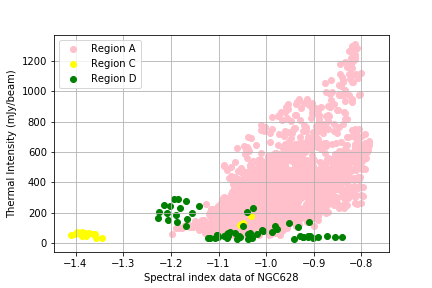
\includegraphics[scale = 0.65]{13Regions_thermal_region_ACandD.png}
	\caption{Correlation of the flux density value with the spectral index map values, for each pixel. The various regions have different 			slops of correlation, which is interesting. This plot shows the regions A, C and D.}
	\label{ngc_acd}
	\end{figure}
	

\section{Making of thermal maps}
To understand how the thermal map is made, one can refer to \citet{2017A&A...600A...6M}. In this section I will explain why a simpple H-$\alpha$ map might not be sufficient if one needs to do an in-depth analysis of thermal emission in the galaxy, and for an accurate determination of the magnetic fields in the galaxy. Classically, the separation of the thermal and non-thermal components has been done by assuming the spectral index of synchrotron emission to be $\alpha_{\text{Syn}}$ = $-$1.0. This method overestimates the amount of thermal emission in the spiral arms, as the $\alpha_{\text{Syn}}$ in such regions is flatter than the assumed value. The $\alpha_{\text{Syn}}$ is also steeper in the inter-arm regions and the outer disk of the galaxy, where a higher amount of synchrotron emission takes place. This leads to an overestimation of the thermal emission in such regions. Another approach is to use 24~$\mu$m infrared (IR) map to estimate the thermal emission. This method also hasa its own set of caviates viz, IR emission may also come from non-thermal sources such as super massive black holes, and energetic cosmic rays (CRs)may also produce IR, thus overestimating the thermal fractionsw in such regions. In this thesis, the thermal map has been made using an extinction corrected H-$\alpha$ map. An H-$\alpha$ map in itself suffers from dust extinction, which would underestimate the amount of thermal emission. In the method where extinction correction is done, the optical depth for the whole galaxy is obtained using high resolution FIR data at 70 and 160~$\mu$m. Using this, one can determine the amount of extinction, thus producing a very good estimate of the thermal tempelate. This method was developed by \citet{2007A&A...475..133T}, and is used in the thermal map that I use in my thesis for NGC\,628. The thermal map for IC\,342 was based on the separation of the thermal and non- thermal components by assuming a constant spectral index, as the extintion corrected thermal map was not available. My thesis does not require an accurate determination of magnetic fields and cosmir ray propagation. Thus, a superficial understanding of the thermal regions in the galaxy was sufficient.
\end{document}
